\subsection{Pharos/TCRD target illumination: how druggable is the gated surfaceome?}
\label{sec:pharos}
DrugCentral (2021 snapshot) and Open Targets gave small-molecule- and
tractability-centric views; Pharos (TCRD, Illuminating the Druggable Genome)
assigns each human protein a Target Development Level (TDL: Tclin = target of
an approved drug with mechanism, including biologics; Tchem = potent
small-molecule ligands; Tbio = biology known, no ligands; Tdark = effectively
unstudied) plus a TIN-X novelty score. We queried the Pharos GraphQL API for
all 205 study genes (202 resolved to a target record; unresolved cases
carried forward as no-record) plus an EGFR sentinel.

\paragraph{Calibration gate.} Pre-registered gates PASSED: (G1) all four CAR-T
reference targets are Tclin (observed 4/4 (CD19=Tclin, ERBB2=Tclin, FOLR1=Tclin, TNFRSF17=Tclin)); (G2) coverage 202/205
resolved records; (G3) at least three of four essential-gene controls are not
Tclin, confirming housekeeping is undrugged in the resource (observed
3/4 (POLR2A=Tbio, RPS3=Tbio, PCNA=Tchem, PSMA1=Tclin)); (G4) the EGFR sentinel is Tclin in both Pharos and DrugCentral
(observed Pharos Tclin, DrugCentral Tclin).

\paragraph{Illumination of gated versus background.} Tclin fraction is
11/99 gated versus 8/95 background (Fisher odds ratio
1.36, $p=0.632$). Full TDL mix gated: Tclin 11, Tchem 24, Tbio 60, Tdark 4; background: Tclin 8, Tchem 16, Tbio 43, Tdark 28. Gated and background genes do not differ in Tclin fraction: clinical illumination is not what separates the panel from a random surface set.
Median TIN-X novelty is 0.0031 (gated) versus 0.015 (background)
(Mann--Whitney $p=8.08e-08$; larger novelty means less studied). Gated antigens are significantly better studied than background, so the panel is not an understudied set on the TIN-X axis.
Median approved-drug count is 0 versus 0 ($p=0.776$) and median
ligand count 0 versus 0 ($p=0.23$).

\paragraph{Cross-source Tclin concordance.} Across 198 genes present in
both resources, Pharos and the 2021 DrugCentral snapshot agree on Tclin status
for 96.0\% (Cohen's $\kappa=0.77$). Discordant genes (8):
ADH1A, ADH1B, ADH1C, ATP1B2, FOLR1, KRAS, TACSTD2, TNFRSF17. The two independent druggability resources substantially agree, so Tclin calls are robust to provenance; named discordances mark post-snapshot approvals or source-specific curation.

\paragraph{AND-gate antigens.} CA9: Tclin, 20 approved drugs, 4185 ligands, novelty 0.00072; CA12: Tclin, 20 approved drugs, 3453 ligands, novelty 0.0034; CLDN18: Tbio, 0 approved drugs, 0 ligands, novelty 0.013; CLDN6: Tbio, 0 approved drugs, 0 ligands, novelty 0.018; MSLN: Tbio, 0 approved drugs, 0 ligands, novelty 0.0019; PSCA: Tbio, 0 approved drugs, 0 ligands, novelty 0.0032; SLC39A6: Tbio, 0 approved drugs, 0 ligands, novelty 0.014.

\begin{figure}[t]
\centering
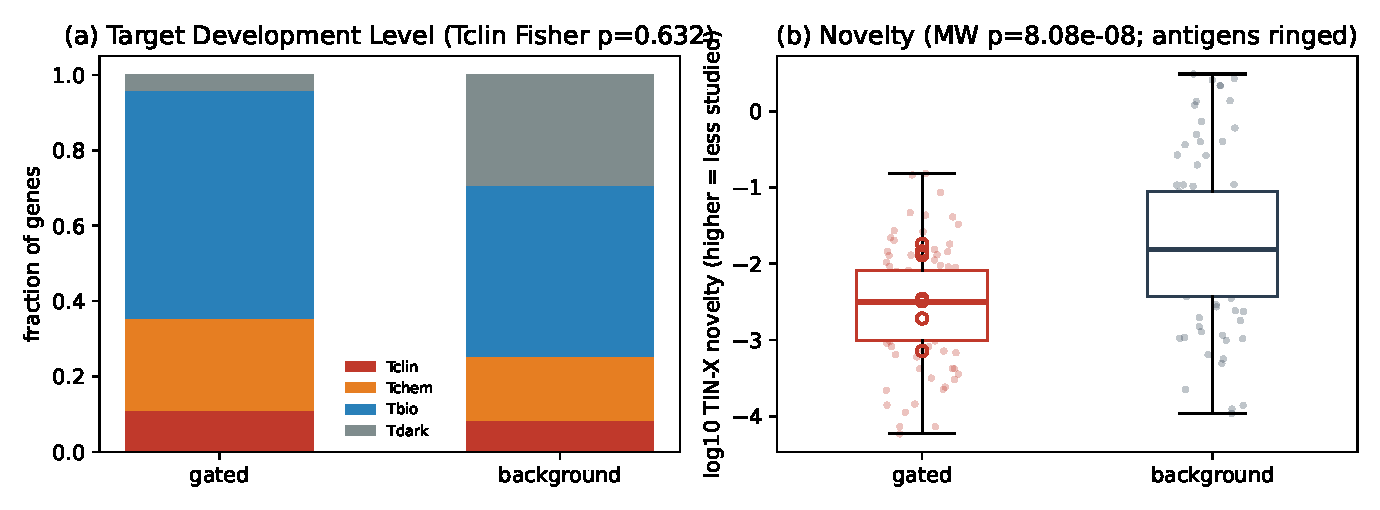
\includegraphics[width=\linewidth]{pharos_fig.pdf}
\caption{Pharos illumination audit. (a) Target Development Level mix for
gated versus background genes. (b) TIN-X novelty distribution (log scale;
higher = less studied), with the seven AND-gate antigens ringed.}
\label{fig:pharos}
\end{figure}
